% ===============================================================
%
%  Template for creating scribe notes for CS:3330, Algorithms.             I am using this template to get my homework PDF's set up as well
%
%  Fill in your name, lecture date, and body of scribe notes
%  as indicated below.
%
% ===============================================================

\documentclass[11pt]{article}

\usepackage{graphicx}
\usepackage{amssymb, amsthm}
\usepackage{pgfplots}
\usepackage{tikz}
\usetikzlibrary{datavisualization}
\usetikzlibrary{datavisualization.formats.functions}
\usepackage{mathtools}
\usepackage{amsmath}
\usepackage{algorithmicx}
\usepackage{algorithm}
\usepackage{algpseudocode}
\usepackage{multirow}



\setlength{\topmargin}{0pt}
\setlength{\textheight}{9in}
\setlength{\headheight}{0pt}
\setlength{\headsep}{0pt}
\setlength{\oddsidemargin}{0.25in}
\setlength{\textwidth}{6in}

\pagestyle{plain}

\begin{document}

\thispagestyle{empty}

\begin{center}
\bf\large CS:3330, Algorithms
\end{center}

\begin{center}
\bf\large HW08 - Dynamic Programming  %Fill in Name of Homework here
\end{center}

\noindent
Logan Zweifel     % FILL IN YOUR NAME HERE
\hfill
September 26, 2021           % FILL IN HW DATE HERE

\noindent
\rule{\textwidth}{1pt}

\medskip

%%%%%%%%%%%%%%%%%%%%%%%%%%%%%%%%%%%%%%%%%%%%%%%%%%%%%%%%%%%%%%%%
% BODY OF HOMEWORK NOTES GOES HERE
%%%%%%%%%%%%%%%%%%%%%%%%%%%%%%%%%%%%%%%%%%%%%%%%%%%%%%%%%%%%%%%%

\section{Binomial Coefficient}
Use the equation

\begin{equation*}
\binom{n}{k} = \frac{n!}{k!(n-k)!}
\end{equation*}

to show

\[ \binom{n}{k} = 
	\begin{cases}
		1		& \quad \text{if } k=0 \text{ or $k=n$} \\
		\binom{n-1}{k-1}+\binom{n-1}{k}	& \quad \text{if } 0<k<n \text{ }
	\end{cases}
\]

\bigskip
\bigskip

For $k=0$,

\begin{eqnarray*}
\frac{n!}{k!(n-k)!} &=& \frac{n!}{0!(n-0)!} \\
	&=& \frac{n!}{1(n)!} \\
	&=& \frac{n!}{n!} \\
	&=& 1
\end{eqnarray*}

\bigskip
\bigskip
\bigskip

For $k=n$,

\begin{eqnarray*}
\frac{n!}{k!(n-k)!} &=& \frac{n!}{n!(n-n)!} \\
	&=& \frac{n!}{n!(0)!} \\
	&=& \frac{n!}{n!} \\
	&=& 1
\end{eqnarray*}


\bigskip
\bigskip
\bigskip

For $0<k<n$, $\binom{n-1}{k-1}$ per the definition of $\binom{n}{k}$ can be simplified to 

\begin{equation*}
\binom{n-1}{k-1} = \frac{(n-1)!}{(k-1)!(n-k-2)!} * \frac{k}{k} =  \frac{k*(n-1)!}{k!(n-k-2)!}
\end{equation*}

and $\binom{n-1}{k}$ can be simplified to

\begin{equation*}
\binom{n-1}{k} = \frac{(n-1)!}{k!(n-k-1)!}
\end{equation*}

\bigskip
\bigskip
\bigskip

\noindent Then the following can be done.

\begin{eqnarray*}
\frac{k*(n-1)!}{k!(n-k-2)!} + \frac{(n-1)!}{k!(n-k-1)!} &=& \frac{(n-1)!}{k!} \left [ \frac{k}{(n-k-2)!} + \frac{1}{(n-k-1)!} \right ] \\
	&=& \frac{(n-1)!}{k!} \left [ \frac{k}{(n-k-2)!} + \frac{1}{(n-k-1)(n-k-2)!} \right ] \\
	&=& \frac{(n-1)!}{k!(n-k-2)!} \left [ k + \frac{1}{n-k-1} \right ] \\
	&=& \frac{(n-1)!}{k!(n-k-2)!}* \frac{k+n-k-1}{n-k-1} \\
	&=& \frac{(n-1)!}{k!(n-k-2)!}* \frac{n-1}{n-k-1} \\
	&=& \frac{n!}{k!(n-k)!}
\end{eqnarray*}

Therefore verifying the recurrence for $\binom{n}{k}$.


\section{Shortest Paths}
Supppose Floyd's algorithm is executed on the graph below

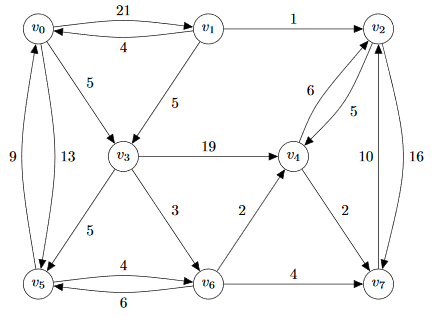
\includegraphics{WeightedGraph.png}

\subsection*{a) Show the contents of the matrix W}

\bigskip
\bigskip

\begin{center}
\begin{tabular} {c c | c c c c c c c c}
	\multicolumn{10}{c}{$v_j$} \\
	\multirow{10}{*}{$v_i$} \\
	& x & 0 & 1 & 2 & 3 & 4 & 5 & 6 & 7 \\
	\hline
	& 0 & 0 & 21 & $\infty$ & 5 & $\infty$ & 13 & $\infty$ & $\infty$ \\
	& 1 & 4 & 0 & 1 & 5 & $\infty$ & $\infty$ & $\infty$ & $\infty$ \\
	& 2 & $\infty$ & $\infty$ & 0 & $\infty$ & 5 & $\infty$ & $\infty$ & 16 \\
	& 3 & $\infty$ & $\infty$ & $\infty$ & 0 & 19 & 5 & 3 & $\infty$ \\
	& 4 & $\infty$ & $\infty$ & 6 & $\infty$ & 0 & $\infty$ & $\infty$ & 2 \\
	& 5 & 9 & $\infty$ & $\infty$ & $\infty$ & $\infty$ & 0 & 4 & $\infty$ \\
	& 6 & $\infty$ & $\infty$ & $\infty$ & $\infty$ & 2 & 6 & 0 & 4 \\
	& 7 & $\infty$ & $\infty$ & 10 & $\infty$ & $\infty$ & $\infty$ & $\infty$ & 0 \\[0.2cm]
	\multicolumn{10}{c}{W} \\ 
\end{tabular}
\end{center}



\subsection*{b) Show the contents of the Matrix D}

\bigskip
\bigskip

\begin{center}
\begin{tabular} {c c | c c c c c c c c}
	\multicolumn{10}{c}{$v_j$} \\
	\multirow{10}{*}{$v_i$} \\
	& x & 0 & 1 & 2 & 3 & 4 & 5 & 6 & 7 \\
	\hline
	& 0 & 0 & 21 & 16 & 5 & 10 & 10 & 8 & 12 \\
	& 1 & 4 & 0 & 1 & 5 & 6 & 10 & 8 & 12 \\
	& 2 & $\infty$ & $\infty$ & 0 & $\infty$ & 5 & $\infty$ & $\infty$ & 7 \\
	& 3 & 14 & 35 & 11 & 0 & 5 & 5 & 3 & 7 \\
	& 4 & $\infty$ & $\infty$ & 6 & $\infty$ & 0 & $\infty$ & $\infty$ & 2 \\
	& 5 & 9 & 30 & 12 & 14 & 6 & 0 & 4 & 8 \\
	& 6 & 15 & 36 & 8 & 20 & 2 & 6 & 0 & 4 \\
	& 7 & $\infty$ & $\infty$ & 10 & $\infty$ & 15 & $\infty$ & $\infty$ & $\infty$ \\[0.2cm]
	\multicolumn{10}{c}{D} \\ 
\end{tabular}
\end{center}

\bigskip
\noindent In this table, $\infty$ represents paths that aren't possible for the given graph because vertexes 2, 4 and 7 are in a permanent cycle and have no way/path to reach other vertices.



\subsection*{c) What is the shortest path from $v_0$ to $v_2$}

\noindent The shortest path from $v_0$ to $v_2$ is $[v_0, v_3, v_6, v_4, v_2]$ with a length/weight of 16.













%%%%%%%%%%%%%%%%%%%%%%%%%%%%%%%%%%%%%%%%%%%%%%%%%%%%%%%%%%%%%%%%

\end{document}